\documentclass{article}

\usepackage[english]{babel}
\usepackage[utf8]{inputenc}
\usepackage{fancyhdr}

\usepackage[a4paper, total={7in, 10in}]{geometry}
\usepackage{graphicx}

\graphicspath{ {./images/} }

\pagestyle{fancy}
\fancyhf{}
\fancyhead[L]{\leftmark}
\fancyhead[R]{\thepage}

% New commands
    \newcommand{\vect}[1]{\left[\begin{array}{c}#1\end{array}\right]}
    \newcommand{\ifcases}[1]{\left\{\begin{array}{cc}#1\end{array}\right.}
% 

\title{Schaltsteller}
\author{Samuel Nösslböck}
\date{May 2022}

\begin{document}

\maketitle

\section{Introduction}

    The following variables are given:
    
    \[
     U_B = 145V \quad \Delta I = I_0 \cdot 2\% \quad t_{ON} = 17.375\mu s \quad f_T = 33kHz \quad R_L = 12.31\Omega 
    \]
    
    Out of these the following constants can be calculated
    \[
    T = \frac{1}{f_T} = 30.3ms
    \]

\section {Voltages over time}

    As a PWN-Signal is used to regulate the current flow in the magnetic coil $L$, the functions for the Voltage are (in the ideal case) discontinuous. 
    The voltage $u_1$ represents the voltage used as a PWM signal:
    
    \begin{equation}
        u_1(t) = \ifcases{5V & \textbf{if}\quad ((t\;\textbf{mod}\; T) \leq t_{ON}) \\ 0V & \textbf{otherwise}}
    \end{equation}
    
    The PWM signal turns the transistor off and on at the given frequency, which causes the current to flow with the base voltage and some losses caused by the transistor. The negative voltage when turned off is created by the diode.
    
    \begin{equation}
        u_E(t) = \ifcases{U_{Emax} & \textbf{if}\quad ((t\;\textbf{mod}\; T) \leq t_{ON}) \\-U_F & \textbf{otherwise}} \quad U_{Emax} = U_B - U_{CEsat} \quad U_{CEsat} = const
    \end{equation}
    
    Here $U_{CEsat}$ and $U_F$ are representing the feed voltages for the transistor and the diode. The voltage on the coil $U_L$ is measured against the (in ideal case) constant voltage of $U_0$, which means the function over time results in: 
    
    \begin{equation}
        u_L(t) \approx u_E(t) - u_0
    \end{equation}
    
\section {Current flow in coil}

    The current in the coil follows two different curves, one when building up the magnetic field, the other when decreasing it. Using the following two equations, magnetism can be described in a very accurate way.
    
    \begin{equation}
        i_{LB}(t) = (I_{max} - I_{start})( 1 - e^{- \frac{t \cdot R}{L}}) + I_{start} \quad
        I_{max} = \frac{U_L}{R_L}
    \end{equation}
    
    \begin{equation}
        i_{LD}(t) = I_{start} \cdot e^{- \frac{t \cdot R}{L}}
    \end{equation}
    
    \textit{( Note: } $I_{start}$ \textit{represents the current in the coil at the start of the build up/decrease )}
    
    \begin{center}
        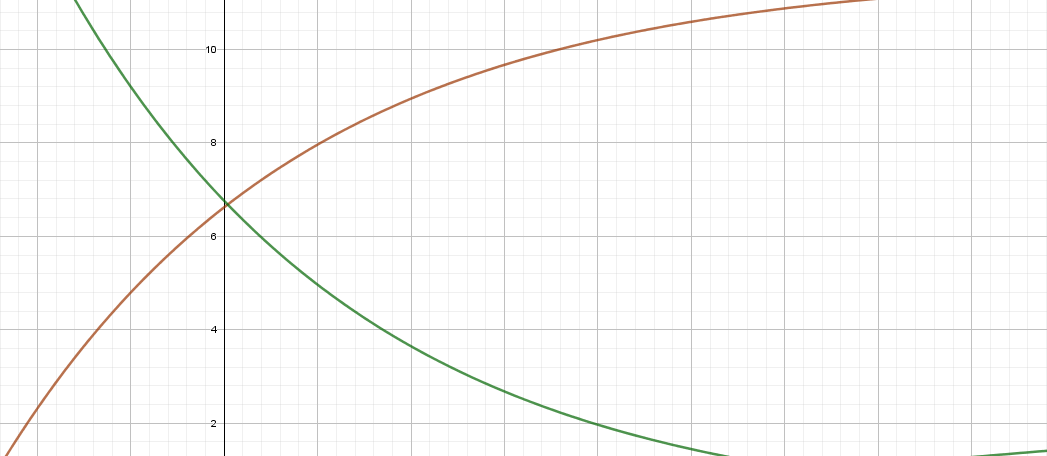
\includegraphics[scale=0.4]{images/IncreaseAndDecrease.PNG}
    \end{center}
    
\section{Solving the current pendulum}
    
    When switching between increasing and decreasing over and over again, the current behaves like a pendulum. At the beginning, this pendulum starts at the value zero and the magnetic field increases faster then it decreases. 
    
    But this higher increase rate slows down the higher $I_0$ gets until it reaches a certain value. This peak value of $I_0$ can be calculated using the ideal case again: 
    
    \begin{equation}
        I_0 = \frac{U_0}{R_L} \quad U_0 \approx v \cdot U_{Emax} - (1 - v) \cdot U_F
    \end{equation}
    
    The pendulum range is expressed by the variable $\Delta I$ and usually as in our case a defined constant. When knowing this pendulum range, the \textbf{defining equation of the pendulum} can be formed:
    
    \begin{equation}
        \Delta I = i_{LB}(t_{ON}) - i_{LB}(0) = - (i_{LD}(t_{OFF}) - i_{LD}(0))
    \end{equation}
    
    \begin{equation}
        \Delta I = (I_{max} - I_{start})(1 - e^{-\frac{t_{ON} R}{L}}) = I_{start}(1 - e^{-\frac{t_{OFF}\cdot R}{L}}) 
    \end{equation}
    
    Out of these two equations, $I_{start}$ and $L$ can be solved
    
    \begin{equation}
        I_{start} = \frac{\Delta I}{1 - e^{-\frac{t_{OFF}\cdot R}{L}}} \quad \Delta I= (I_{max} - \frac{\Delta I}{1 - e^{-\frac{t_{OFF}\cdot R}{L}}})(1 - e^{-\frac{t_{ON} R}{L}})
    \end{equation}
    
    Out of this function $L$ can be solved numerically: 
        
    \[
        L \approx 7.98mH \quad I_{start} \approx 6.63A
    \]
    
    \begin{center}
        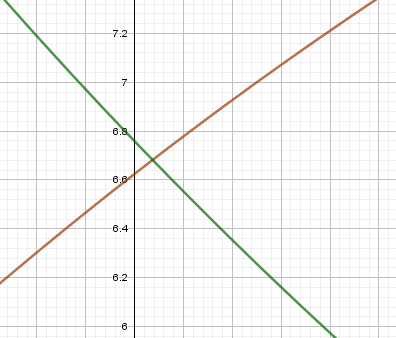
\includegraphics[scale=0.75]{images/CurrentPendulum.PNG}
    \end{center}
    
    Notice how the curves approach a linear form at this clock speed, which results in a highly stable voltage output and a high accuracy of linear approximations. 
        
\end{document}